\section{Theoretical Analysis}
\label{sec:analysis}

In this section we will analyse theoretical our audio amplifier circuit. \\
To do so, and because there were several things to be analysed, we divided the theoretical analysis in the following subsections that explain the different sectors that our circuit has and also each one will be detailed separately.\\

\begin{figure}[H] 
\centering
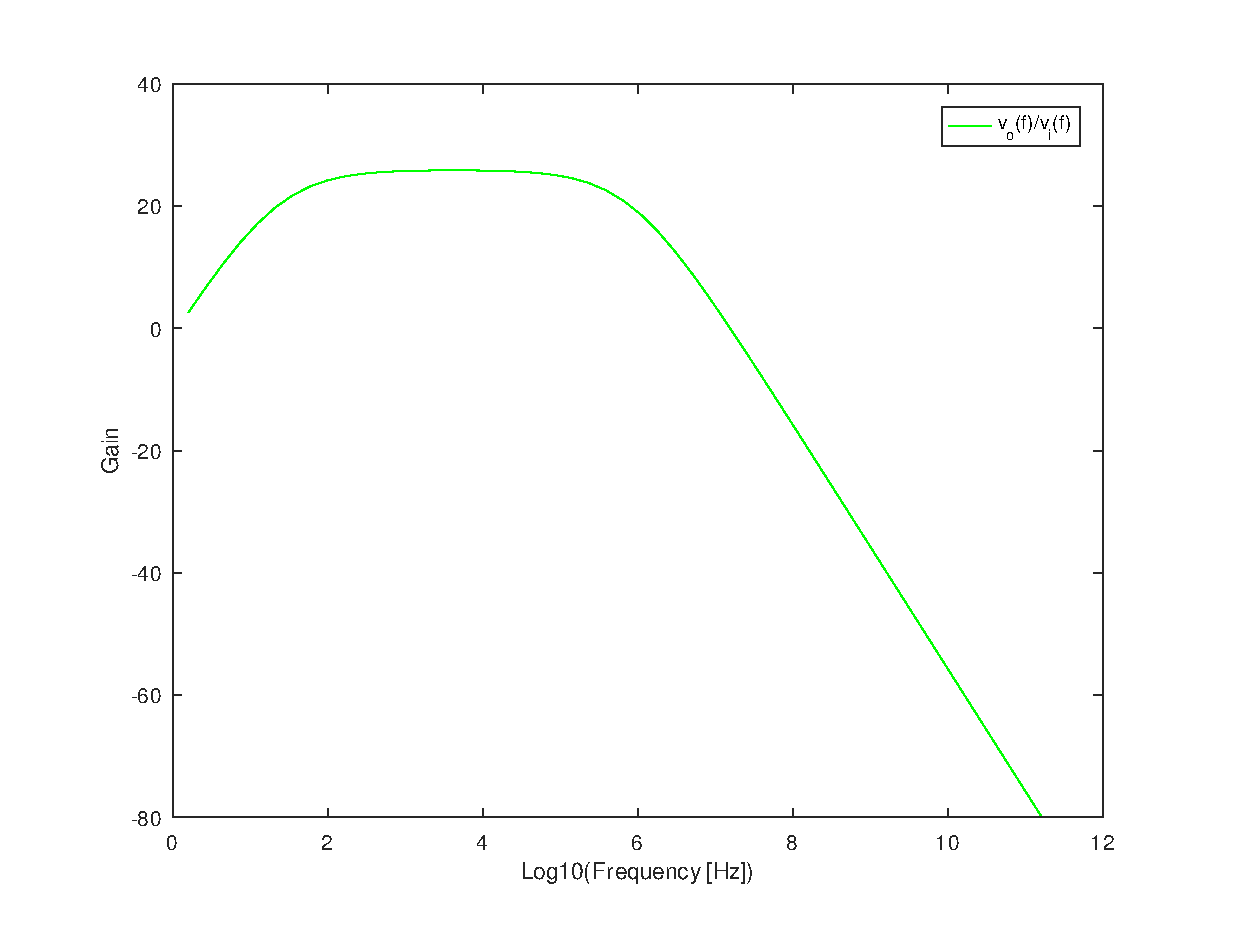
\includegraphics[width = 8cm]{Gain.eps} 
\caption{Gain}
\label{gain}
\end{figure}

\begin{figure}[H] 
\centering
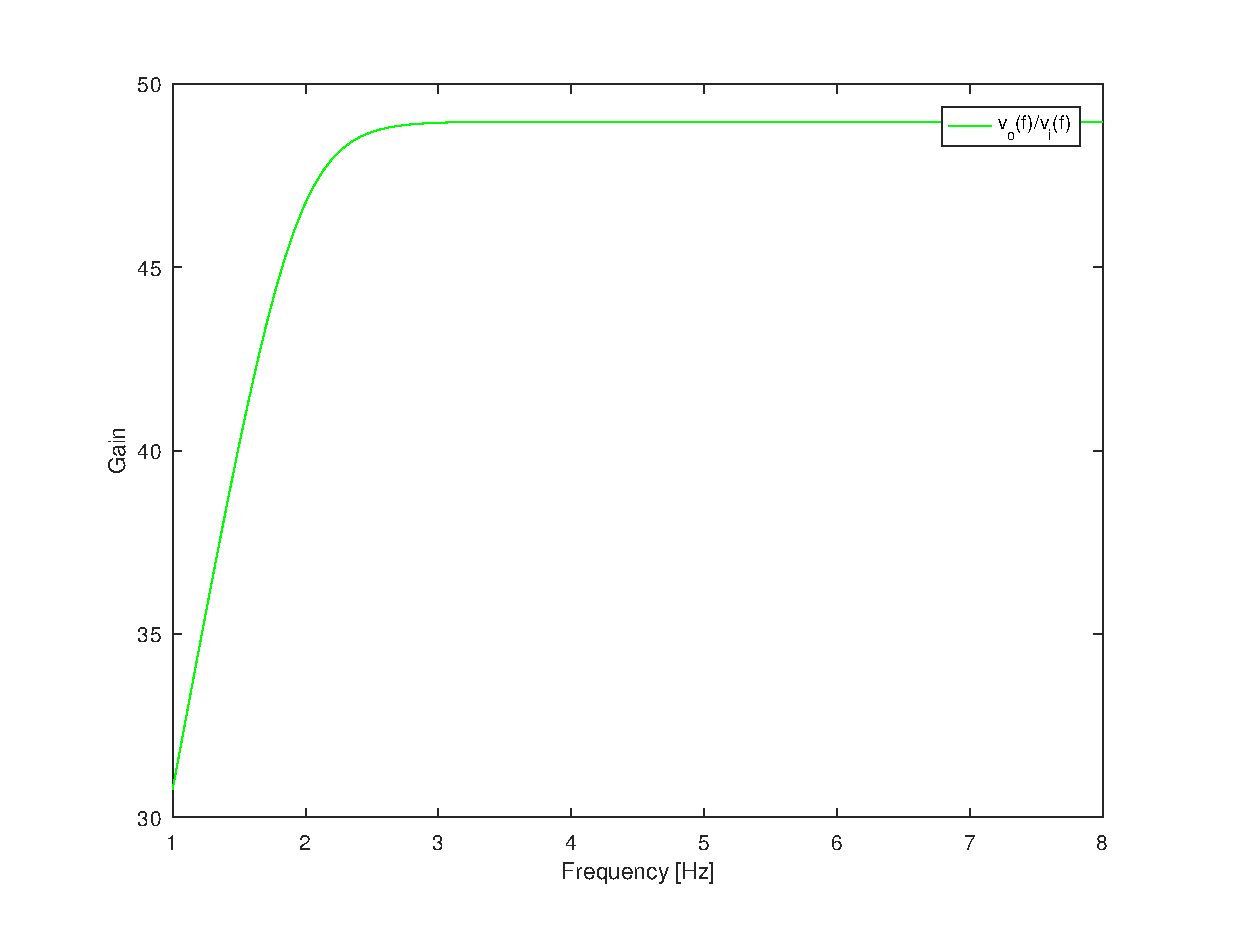
\includegraphics[width = 8cm]{Output.eps} 
\caption{Output}
\label{output}
\end{figure}

\begin{table}[H] \centering
\begin{tabular}{|
>{\columncolor[HTML]{FFCC67}}l |c|}
\hline
\multicolumn{2}{|l|}{\cellcolor[HTML]{EABD8B}Name - Value} \\ \hline
@gb[i] & -2.86455e-04\\ \hline
@r1[i] & 2.732477e-04\\ \hline
@r2[i] & -2.86455e-04\\ \hline
@r3[i] & -1.32073e-05\\ \hline
@r4[i] & 1.229564e-03\\ \hline
@r5[i] & -2.86455e-04\\ \hline
@r6[i] & 9.563162e-04\\ \hline
@r7[i] & 9.563162e-04\\ \hline
v(1) & 5.216040e+00\\ \hline
v(2) & 4.939074e+00\\ \hline
v(3) & 4.361415e+00\\ \hline
v(5) & 4.978786e+00\\ \hline
v(6) & 5.853598e+00\\ \hline
v(7) & -2.00109e+00\\ \hline
v(8) & -2.97875e+00\\ \hline
v(9) & 0.000000e+00\\ \hline

\end{tabular}
\caption{optab}
\end{table}

\begin{table}[H] \centering
\begin{tabular}{|
>{\columncolor[HTML]{FFCC67}}l |c|}
\hline
\multicolumn{2}{|l|}{\cellcolor[HTML]{EABD8B}Name - Value} \\ \hline
First Stage\\ \hline
AV1-DB & 2.634352e+01 dB\\ \hline
ZI1 & 2.811209e+03 Omega \\ \hline
ZO1 & 3.754073e+03 Omega \\ \hline
Second Stage\\ \hline
AV2-DB & -7.252308e-02 dB\\ \hline
ZI2 & 4.075483e+04 Omega \\ \hline
ZO2 & 1.478440e+00 Omega \\ \hline
Complete\\ \hline
ZO & 1.710806e+01 Omega\\ \hline
AV-DB & 2.593695e+01 dB\\ \hline
Merit & 4.398471e+02 \\ \hline
HighCutOff frequency & 8.304945e+05 Hz\\ \hline
LowCutOff frequency & 2.183854e+01 Hz\\ \hline
Cost & 2.242430e+03 MU's\\ \hline
Bandwidth & 8.304726e+05 rad/s\\ \hline

\end{tabular}
\caption{Point 2}
\end{table}

